\section{Анализ полученных данных}
\label{sec:analysis}

В данной описывается влияние параметров системы на сжатие изображений.
Параметры влияние которых исследовалось:

\begin{itemize}
  \item частота дискретизации;
  \item количество входных нейронов сети;
  \item количество нейронов на самом узком участке нейронной сети;
  \item количество тестовых примеров, подобранных для обучения сети.
\end{itemize}

В итоге был сформирован такой набор тестов:

\begin{itemize}
  \item 3 глубины дискретизации изображения(8,32 и 256 уровней);
  \item 4 множества входных нейронов сети(16, 25, 64 и 100 нейронов);
  \item 6 отношений количества нейронов на самом узком участке сети к количеству входных нейронов(2 к 8, 3 к 8, 4 к 8, 5 к 8, 6 к 8 и 7 к 8);
  \item 15 наборов тестов к каждому обучению сети в количестве от 10 до 150 с шагом 10.
\end{itemize}

Было проведено 7560 тестов. Процесс был расспараллен на все вычислительные потоки центрального процессора.
Каждый поток обрабатывал тесты для одного изображения и сохранял данные о результатах тестирования в тектовый файл,
но вычисления все равно заняли 5 суток процессорного времени.
Программа собирала данные о времени затраченном на сжатие изображения в конкретном тесте, степень сжатия,
соотношение сигнал-шум и среднеквадратическое отклонение для исходного и полученного изображения.
Так же программа сохраняла изображение в сжатом виде и его декодированную версию.

\subsection{Частота дискретизации}
\label{sub:analysis:discrete}
С процессом квантования и дискретизации связано понятие визуальной избыточности.
Значительная часть информации на изображении не может быть воспринята человеком:
например, человек способен замечать незначительные перепады яркости,
но гораздо менее чувствителен к цветности. Также, начиная с определённого момента,
повышение точности дискретизации не влияет на визуальное восприятие изображения.
Таким образом, некоторая часть информации может быть удалена без ухудшения визуального качества.
Такую информацию называют визуально избыточной. Самым простым способом удаления визуальной
избыточности является уменьшение точности дискретизации, но на практике этот способ можно
применять только для изображений с простой структурой, т.к. искажения, возникающие на сложных изображениях, слишком заметны.

Как видно на рисунке~\ref{fig:by_converter_msc} и рисунке~\ref{fig:by_converter_snr},
увеличение глубины дескритезации положительно сказывается на качестве изображения.
Это связано с тем, что нейронная сеть обучается на примерах, более приблеженных к исходному изображению.
В противовес к этому нейронная должна запомнить больше количество комбинаций и построить более сложные связи.

Внимательно изучив полученные изображения, можно заметить, что на сжатых изображениях возникают отчётливые ложные контуры,
которые значительно ухудшают визуальное восприятие. Существуют методы, основанные на переносе ошибки квантования в следующий пиксел,
позволяющие значительно уменьшить или даже совсем удалить эти контуры, но они приводят к зашумлению изображения и появлению зернистости.
Перечисленные недостатки сильно ограничивают прямое применение квантования для сжатия изображений.

\begin{figure}[ht]
\centering
  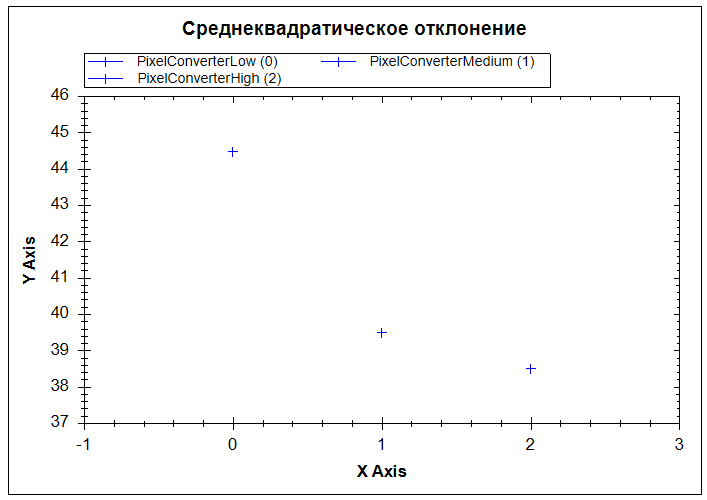
\includegraphics[scale=0.33]{ByConverterMSC.png}
  \caption{ зависимость значений среднеквадратичного отклонения от глубины дискретизации }
  \label{fig:by_converter_msc}
\end{figure}

\begin{figure}[ht]
\centering
  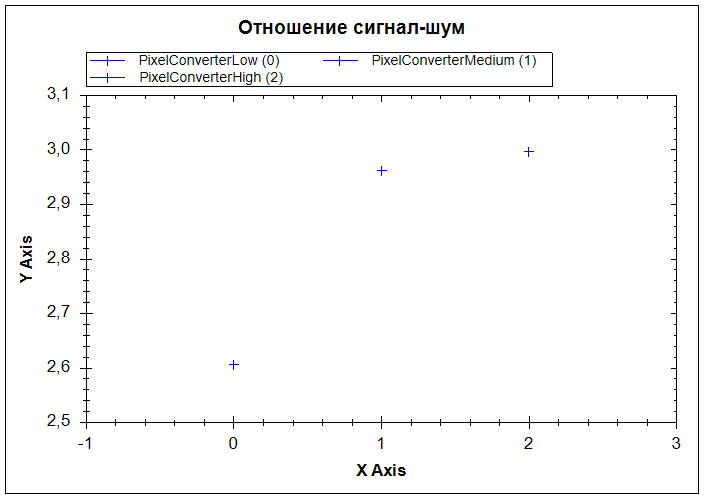
\includegraphics[scale=0.33]{ByConverterSNR.png}
  \caption{ зависимость значений отношения сигнал-шум от глубины дискретизации }
  \label{fig:by_converter_snr}
\end{figure}

Если посмотреть на рисунок~\ref{fig:by_converter_build_time}, то можно заметить переходный этап, когда при достижении определенной
глубины дикретизации, нейронная сеть обучается быстрее. Возможно это связано с тем, что на малой глубине дискретизации,
нейронная сеть запоминает наборы сигналов поступивших на вход. На большой глубине дискретизации, нейронная сеть строит более сложные зависимости
между нейронами и лучше анализирует значение сигнала в зависимости от его положения. А на переходном этапе, нейронная сеть обучается с большим количеством ошибок.
В связи с этим алгоритм снижает скорость обучения сети, чтобы допускать меньше ошибок, приблежение к оптиманьной ошибке затягивается.
В дальнейшем планируется провести больше тестов в данном направлении, потому что из-за ограничений по времени, не удалось охватить больше
уровней глубины дискретизации.

\begin{figure}[ht]
\centering
  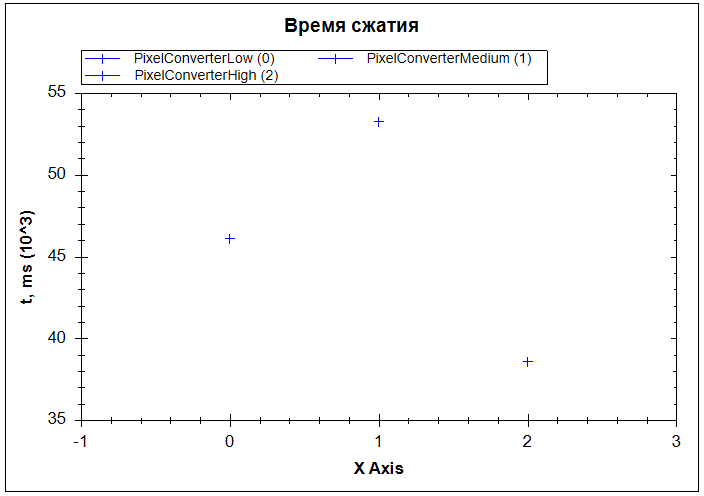
\includegraphics[scale=0.33]{ByConverterBuildTime.png}
  \caption{ зависимость времени сжатия от глубины дискретизации }
  \label{fig:by_converter_build_time}
\end{figure}

На рисунке~\ref{fig:by_converter_size} видно, что с увеличением глубины дискретизации увелеличивается и размер сжатой информации.
Это объясняется тем что после обработки изображения нейронной сетью, получается набор сигналов, который с повышением глубины дискретизации
принимает более детальные значение. То есть повышение глубины дискретизации приводит к увеличению количества комбинаций выходных данных,
а так как на последнем этапе, сигналы сжимаются методом сжатия без потерь, то это приводит к увеличению энтропии, а следовательно и к увеличению
размера выходного набора данных.

\begin{figure}[ht]
\centering
  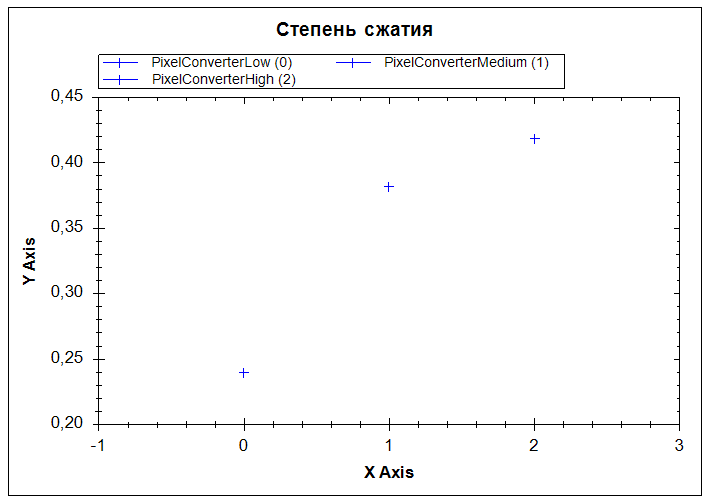
\includegraphics[scale=0.33]{ByConverterSize.png}
  \caption{ зависимость отношения итогового размера к исходному размеру от глубины дискретизации }
  \label{fig:by_converter_size}
\end{figure}

В данном случае использовался алгоритм Хаффмана. Это адаптивный жадный алгоритм оптимального префиксного
кодирования алфавита с минимальной избыточностью. Был разработан в 1952 году аспирантом Массачусетского технологического
института Дэвидом Хаффманом при написании им курсовой работы. В настоящее время используется во многих программах сжатия данных~\cite{kormen}.

\subsection{Размер входного блока}
\label{sub:analysis:input}

Если посмотреть на рисунок~\ref{fig:by_input_msc} видно, что разброс результатов не превышает 2 пунктов. Пункты отражают насколько
один пиксель текущего изображения отличается от пикселя сжатого изображения. Отношение сигнал-шум тоже имеет отклонение не более 0.2 пункта(рисунок~\ref{fig:by_input_snr}).
Это приводит к выводу, что размер блоков слабо влияет на итоговое изображение. Основной критерии выбора размера блока можно вывести следующие:
\begin{itemize}
  \item размер блока должет позволять построить оптимальный набор тестов для обучения;
  \item размер блока не должен быть вырожденным(размеров в 1-4 сигнала);
  \item размер блока должен позволять разбить исходное изображение на оптимальное количество участков,
  по которым, можно будет восстановить исходное изображение.
\end{itemize}

\begin{figure}[ht]
\centering
  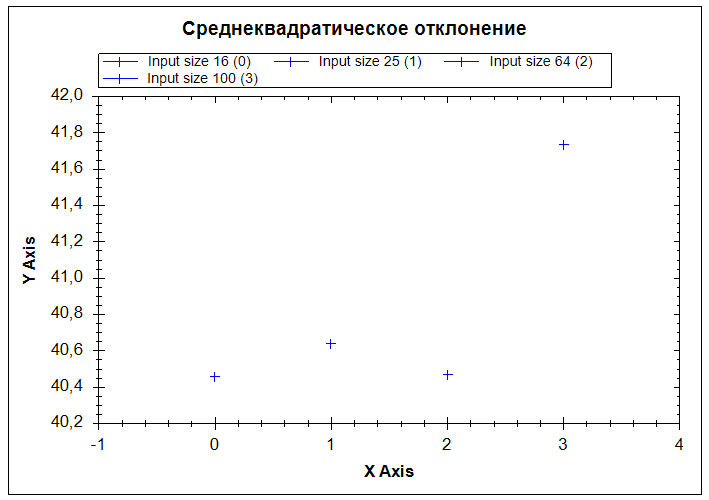
\includegraphics[scale=0.33]{ByInputMSC.png}
  \caption{ зависимость значений среднеквадратичного отклонения от количества нейроннов на входном слое }
  \label{fig:by_input_msc}
\end{figure}

\begin{figure}[ht]
\centering
  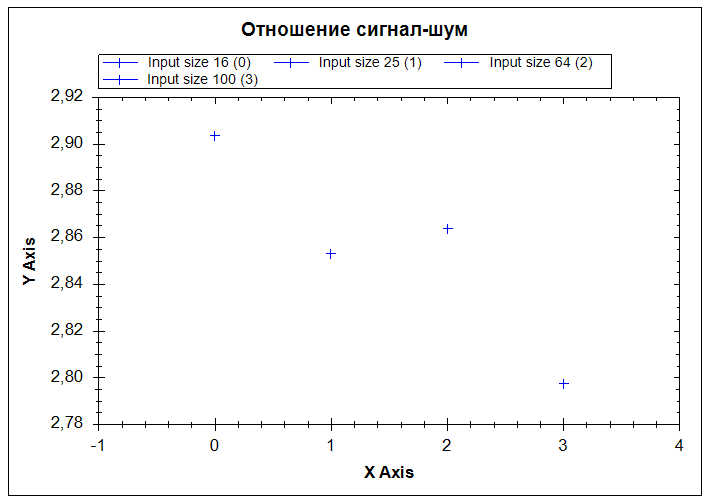
\includegraphics[scale=0.33]{ByInputSNR.png}
  \caption{ зависимость значений отношения сигнал-шум от количества нейроннов на входном слое }
  \label{fig:by_input_snr}
\end{figure}

Фактически сеть с большим количеством нейронов сможет построить более сложные зависимости, между участками изображения,
но подбор тестовых данных и обучение такой сети может занять продолжительное время. Следовательно необходимо найти оптимальное
соотношение времени-сложности сжатия. На рисунке~\ref{fig:by_input_build_time} прослеживается линейная зависимость времени сжатия изобраения
от величины входного слоя. Следовательно оптимальным решением будет брать размер блока меньше, но не слишком маленьким, чтобы нейронная сеть
смогла объективно обучится на выбранных тестах.

\begin{figure}[ht]
\centering
  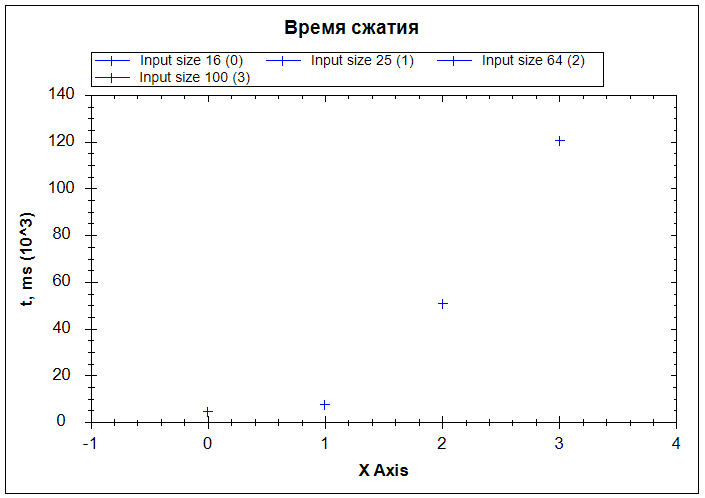
\includegraphics[scale=0.33]{ByInputBuildTime.png}
  \caption{ зависимость времени сжатия от количества нейроннов на входном слое }
  \label{fig:by_input_build_time}
\end{figure}

На рисунке~\ref{fig:by_input_size} видно, что размер входного блока имеет сильное влияние на размер выходных данных.
Очевидно что блок большего размера имеет большее количество возможных представлений и количество их растет экспонинциально.
Это является еще одной причиной, почему следует использовать блоки меньшего размера.

\begin{figure}[ht]
\centering
  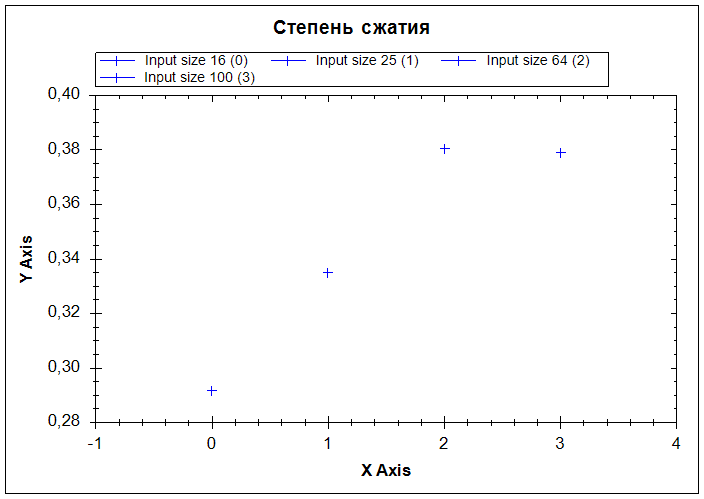
\includegraphics[scale=0.33]{ByInputSize.png}
  \caption{ зависимость отношения итогового размера к исходному размеру от количества нейроннов на входном слое }
  \label{fig:by_input_size}
\end{figure}

Одна из наиболее серьезных трудностей изложенного подхода в том,
что таким образом мы минимизируем не ту ошибку, которую на самом деле нужно минимизировать. В конечном итоге требуется уменьшать ошибку,
которую можно ожидать от сети, когда ей будут подаваться совершенно новые наблюдения. Иначе говоря, чтобы нейронная сеть
обладала способностью обобщать результат на новые наблюдения. В действительности сеть обучается минимизировать ошибку на обучающем множестве,
и в отсутствие идеального и бесконечно большого обучающего множества это совсем не то же самое, что минимизировать требуемую ошибку на поверхности
ошибок в заранее неизвестной модели явления. То есть обучая сеть на заданной выборке блоков, неинзвестно, уменьшается ли ошибка для блоков,
которые будут кодироваться в конечном итоге, для получения сжатого изображения.

\subsection{Соотношение количества нейронов между слоями}
\label{sub:analysis:output}

Если посмотреть на рисунок~\ref{fig:by_output_msc} видно, что разброс результатов не превышает 3 пунктов. Это значит, что соотношение количества нейронов
сильнее влияет на качество итогового изображения, чем размер входного слоя нейроном. Отношение сигнал-шум тоже имеет отклонение не более 0.1 пункта(рисунок~\ref{fig:by_output_snr}).
Из этого можно сделать вывод, что увеличение количества нейроном промежуточного слоя, повышает качество изображения, а из этого следует, что данное оотношение влияет на:
\begin{itemize}
  \item качество изображения;
  \item скорость сжатия;
  \item размер сжатых данных.
\end{itemize}

\begin{figure}[ht]
\centering
  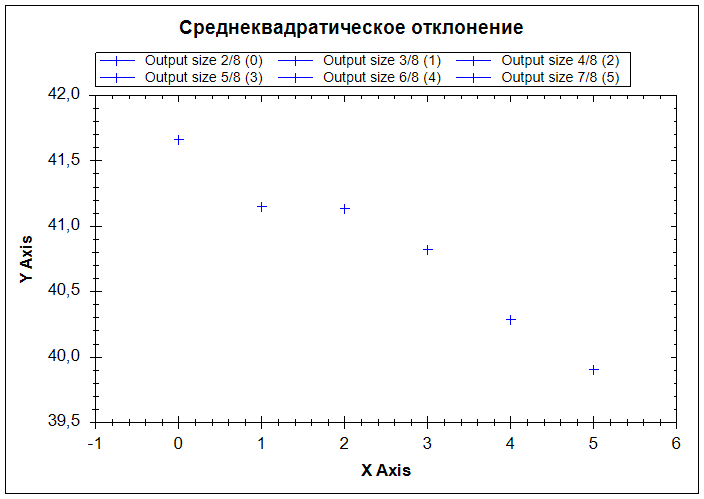
\includegraphics[scale=0.33]{ByOutputMSC.png}
  \caption{ зависимость значений среднеквадратичного отклонения от отношений количества нейронов на слоях }
  \label{fig:by_output_msc}
\end{figure}

\begin{figure}[ht]
\centering
  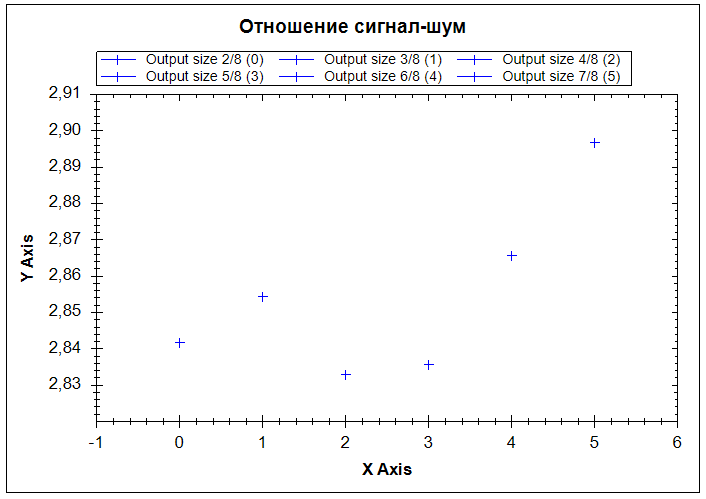
\includegraphics[scale=0.33]{ByOutputSNR.png}
  \caption{ зависимость значений отношения сигнал-шум от отношений количества нейронов на слоях }
  \label{fig:by_output_snr}
\end{figure}

На рисунке~\ref{fig:by_output_build_time} прослеживается сильная зависимость скорости сжатия от данного соотношения.
Это связано с тем, что увеличение количества нейронов в слое приводит к увеличению связей между соседними слоями нейронной сети.
При добавлении одного нейрона в слой, происходит формирование потоков сигналов от всех нейронов предыдущего слоя к новому нейрону.
И для нового нейрона создаются потоки, которые отправляют сигнал от него ко всем нейронам следующего слоя.

\begin{figure}[ht]
\centering
  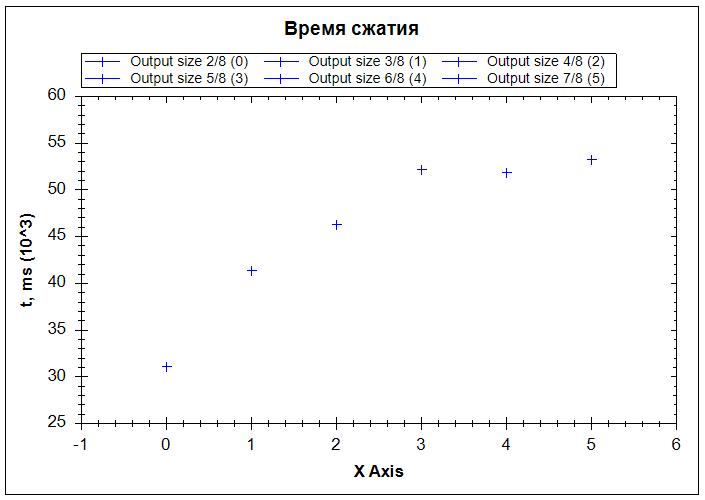
\includegraphics[scale=0.33]{ByOutputBuildTime.png}
  \caption{ зависимость времени сжатия от отношений количества нейронов на слоях }
  \label{fig:by_output_build_time}
\end{figure}

На рисунке~\ref{fig:by_output_size} видно, что соотношение имеет заметное влияние на рамер выходного файла.
Это объясняется тем что после обработки изображения нейронной сетью, получается набор сигналов, который с позволяет запомнить большее количество комбинаций,
полученных из исходного изображения. Так же при увеличении количества нейронов увеличивается размер нейронной сети. Вместе с выходными сигналами хранятся
данные для востановления декодера, а декодер является половиной исходной нейронной сети, полученной в процессе обучения на текущем изображении. Следовательно, чем
больше нейронов и слоёв содержит нейронная сеть, тем больше будет занимать место декодер в выходных данных.

Если весовые коэффициенты к элементам скрытого слоя фиксированы, то необходимо, чтобы количество элементов скрытого слоя экспоненциально возрастало
с ростом размерности задачи. Тем самым, теряется их основное преимущество --- способность решать задачи произвольной сложности при помощи простых элементов.
В данном случае это проявляется в том, что при увеличении размеров входного слоя увеличивается и размер скрытого слоя.

\begin{figure}[ht]
\centering
  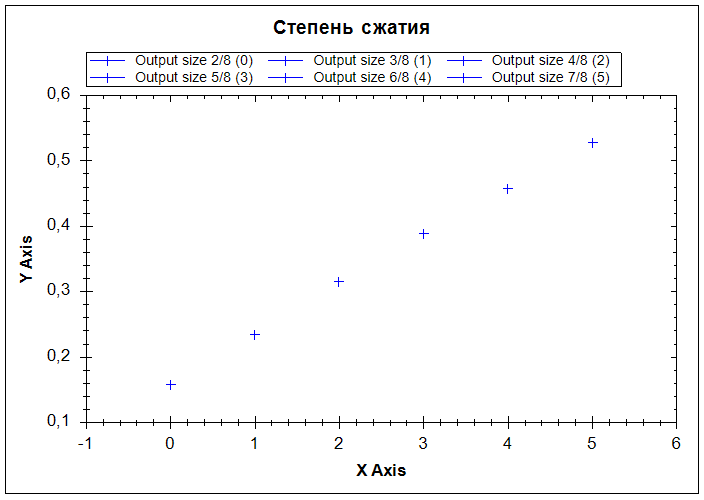
\includegraphics[scale=0.33]{ByOutputSize.png}
  \caption{ зависимость отношения итогового размера к исходному размеру от отношений количества нейронов на слоях }
  \label{fig:by_output_size}
\end{figure}

В отличие от традиционных методов сжатия --- математического вычисления и удаления избыточности --- данная нейронная сеть при решении задачи сжатия исходит
из соображений нехватки ресурсов. Топология сети и ее алгоритм обучения таковы, что данные большой размерности передаются на входной слой нейронов.
Далее сигналы передаются на скрытый слой, который меньше по размеру чем входной слой. Сигналы с скрытого слоя направляются к выходному слою, который
копирует размер входного слоя. В итоге нейронная сеть, состоящая из 3 слоев, напоминает по форме песочные часы.
Слой входных нейронов называется кодером, а слой выходных нейронов называется декодером.
Число промежуточных слоев определяет степень сложности преобразования данных.
апример сеть с тремя промежуточными слоями может выполнять лучшее сжатие на обучающих блоках,
но может дать худший результат в реальных ситуациях. Это связано с тем, что в исходных данных может случайно образоваться некая зависимость,
которая не имеет никакого отношения к реальности.

Веса нейронов были представлены вещественными числами двойной точности, а следовательно занимали 8 байт информации.
Максимальный размер сети, который использовался в данном проекте содержал 880 000 отдельнях весов. Для декодера было необходима только половина этих весов.
Следовательно имеелось 440 000 чисел, занимающих в памяти по 8 байт. При сохранении число байт под отдельное значение веса сокращалось, по причине того, что в данном
случае не требуется точность в 15-16 знаков после запятой, которую дает вещественное число двойной точности. Общий размер декодера занимал значительное количество места в итоговых данных.

\subsection{Количество тестов для обучения нейронной сети}
\label{sub:analysis:tests}

Анализируя данные, полученные на рисунке~\ref{fig:by_tests_count_msc} и рисунке~\ref{fig:by_tests_count_snr},
делаются выводы о том, что увеличение тестов ведет к увеличению величины ошибки.
Это связано с тем, что нейронная сеть начинает специализироваться на конкретных примерах, что дает ошибку на реальных данных.

Переобучение в машинном обучении и статистике --- явление, когда построенная модель хорошо объясняет примеры из обучающей выборки,
но относительно плохо работает на примерах, не участвовавших в обучении (блоки выбранные из исходного изображения).
Это связано с тем, что при построении модели в обучающей выборке обнаруживаются некоторые случайные закономерности,
которые отсутствуют в генеральной совокупности.
Даже тогда, когда обученная модель не имеет чрезмерного количества параметров, можно ожидать, что эффективность её на новых данных будет ниже,
чем на данных, использовавшихся для обучения. В частности, значение коэффициента детерминации будет сокращаться по сравнению с исходными данными обучения.

С переобучением в данном случае, можно бороться увеличением размера нейронной сети. То есть необходимо увеличить количество нейронов на входном слое,
увеличить количество скрытых слоев и число нейронов в них. Тогда нейронная сеть будет способна запомнить большее количество тестов и остаться при этом
не переобученной и способной находить и поддерживать необходимый уровень качества обработки сигналов. Еще один способ борьбы с переобучением,
это подбирать другие данные для обучения, когда достигается определенный порог точности, потому что мы будем использовать обученную нейронную сеть, на данных,
которые нам заранее известны.

\begin{figure}[ht]
\centering
  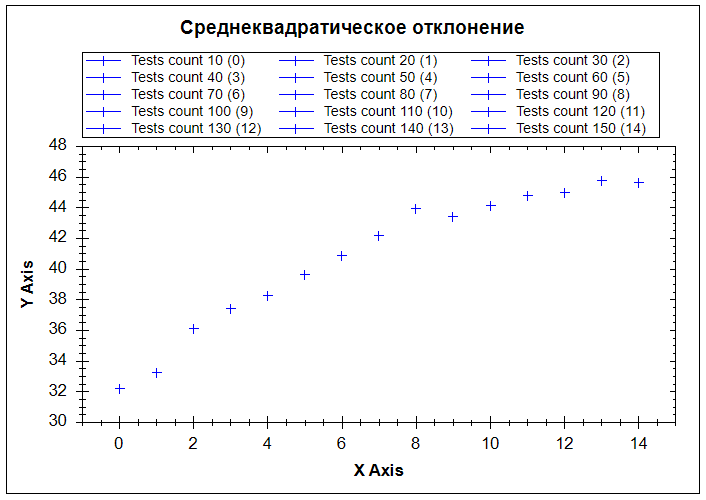
\includegraphics[scale=0.33]{ByTestsCountMSC.png}
  \caption{ зависимость значений среднеквадратичного отклонения от размера данных для обучения нейронной сети }
  \label{fig:by_tests_count_msc}
\end{figure}

\begin{figure}[ht]
\centering
  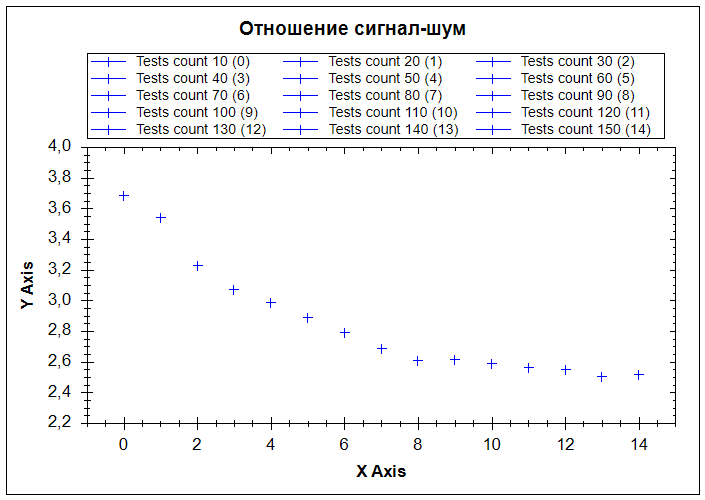
\includegraphics[scale=0.33]{ByTestsCountSNR.png}
  \caption{ зависимость значений отношения сигнал-шум от размера данных для обучения нейронной сети }
  \label{fig:by_tests_count_snr}
\end{figure}

Очевидно, что увеличение количества блоков в тестовом наборе, приводит к увеличению времени обучения(рисунок~\ref{fig:by_tests_count_build_time}).
Это объясняется тем, что нейронной сети требуется сформировать большее количество связей между нейронами. Так же в процессе обучения могут возникать ошибки,
которые задерживают процесс схождения обучения нейронной сети. Даже если процесс обучения не сойдется за обозримое время, в алгоритме было предусмотрено,
что при достижении определенного количества поколений обучения, прерывать процесс. Так как проводилось тестирование параметров сети в разнообразных ситуациях,
получиваяся нейронная сеть, даже не достигнувшая необходимой точности, в любом случае включалась в процесс сжатия изображения. В любом случае требуется следить
за состоянием нейронной сети, тщательно подбирать ее параметры.

После выбора общей структуры нужно экспериментально подобрать параметры сети.
Для сетей, подобных перцептрону, это будет число слоев, наличие или отсутствие обходных соединений, активационные функции нейронов.
При выборе количества слоев и нейронов в них следует исходить из того, что способности сети к обобщению тем выше, чем больше суммарное число
связей между нейронами. С другой стороны, число связей ограничено сверху количеством записей в обучающих данных.

В процессе обучения сеть в определенном порядке просматривает обучающую выборку блоков. Порядок просмотра может быть последовательным, случайным и т. д.
Основной принцип обучения в данном случае заключался в том, что на вход подавались данные, которые и ожидались на выходе. Этот факт значительно облегчает процесс обучения.

\begin{figure}[ht]
\centering
  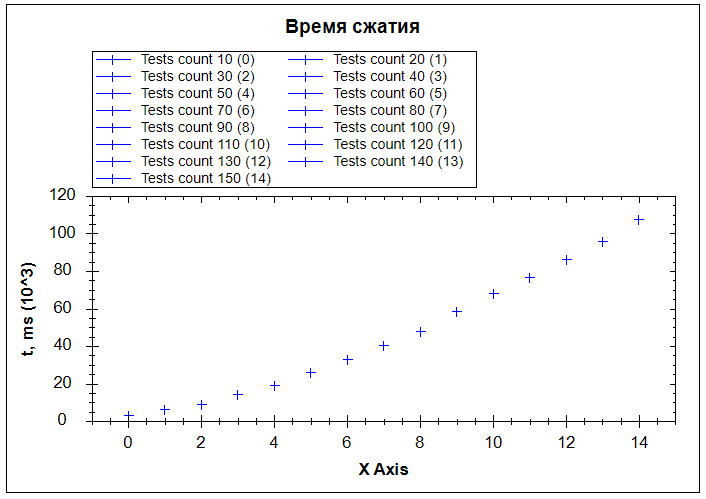
\includegraphics[scale=0.33]{ByTestsCountBuildTime.png}
  \caption{ зависимость времени сжатия от размера данных для обучения нейронной сети }
  \label{fig:by_tests_count_build_time}
\end{figure}

Размер выходных файлов так же зависел от количества блоков, которые были выбраны для обучения(рисунок~\ref{fig:by_tests_count_size}).

\begin{figure}[ht]
\centering
  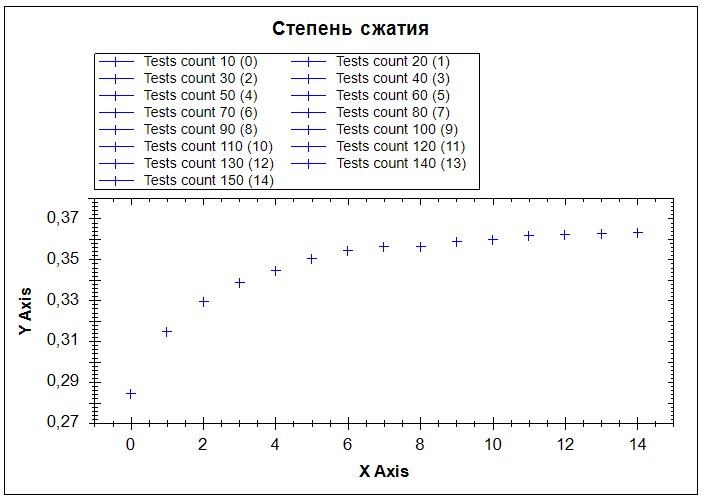
\includegraphics[scale=0.33]{ByTestsCountSize.png}
  \caption{ зависимость отношения итогового размера к исходному размеру от размера данных для обучения нейронной сети }
  \label{fig:by_tests_count_size}
\end{figure}

При увеличении количества тестов происходило увеличение размера выходных данных. Это объясняется увеличением количества комблинаций выходных блоков,
образованных нейронной сетью под влиянием теста с большим количеством блоков.

Таким образом были перечислены основные факторы влияющие на результать кодирования исходных изображений.
